\chapter{Scale laws}\label{ch:scalelaws}
One of the goals of this work is to search, reveal, study and use universal laws in bulk gene expression data.\nocite{altmann2016statistical}
As in chapter~\ref{ch:structure} approaches from different field of science are considered at this point.

In can be interesting to study the behaviour of the gene expression across samples.

\draft{taylor \cite{Eisler2008} }
\section{Scaling}
\draft{gene expression across samples? gamma?}

Given a matrix of components and realisations as~\ref{fig:componetstable} with expression entries $n_{i j}$ it is possible to estimate the mean of a row $m_i=\avg{n_{ij}}_j$ and its variance $\sigma^2_i=\avg{n_{ij}^2}_j - \avg{n_{ij}}^2_j$.

First of all it could be interesting to represent the variance of expression $\sigma^2$ versus 
the average $m$ across tissues.

%%all genes
\begin{figure}[htb!]
    \centering
    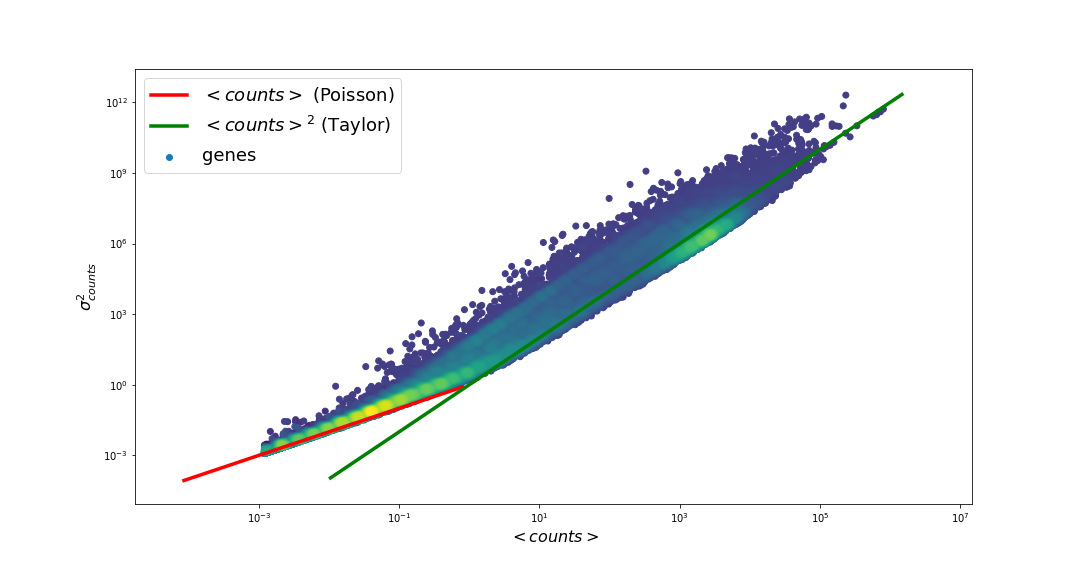
\includegraphics[width=0.9\linewidth]{pictures/scalelaws/gtex/allgenes/varmean_loglog.png}
    \caption{Variance versus occurrence}
    \label{fig:scalelaws/gtex/allgenes/varmean_loglog_density}
\end{figure}

\begin{figure}[htb!]
    \centering
    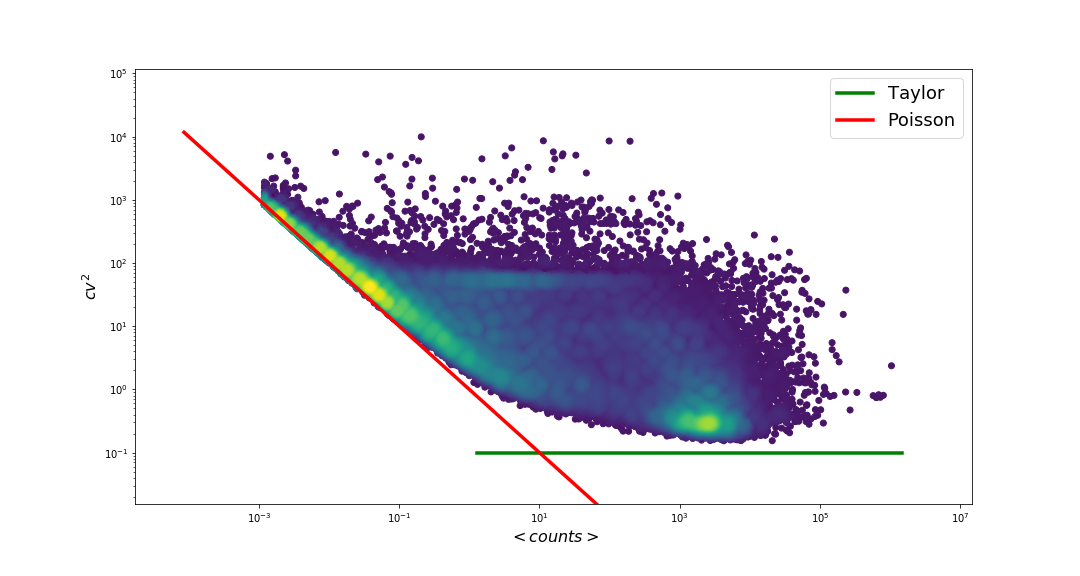
\includegraphics[width=0.9\linewidth]{pictures/scalelaws/gtex/allgenes/cvmean_loglog.png}
    \caption{Variance versus occurrence}
    \label{fig:scalelaws/gtex/allgenes/cvmean_loglog}
\end{figure}

%%protein coding

\begin{figure}[htb!]
    \centering
    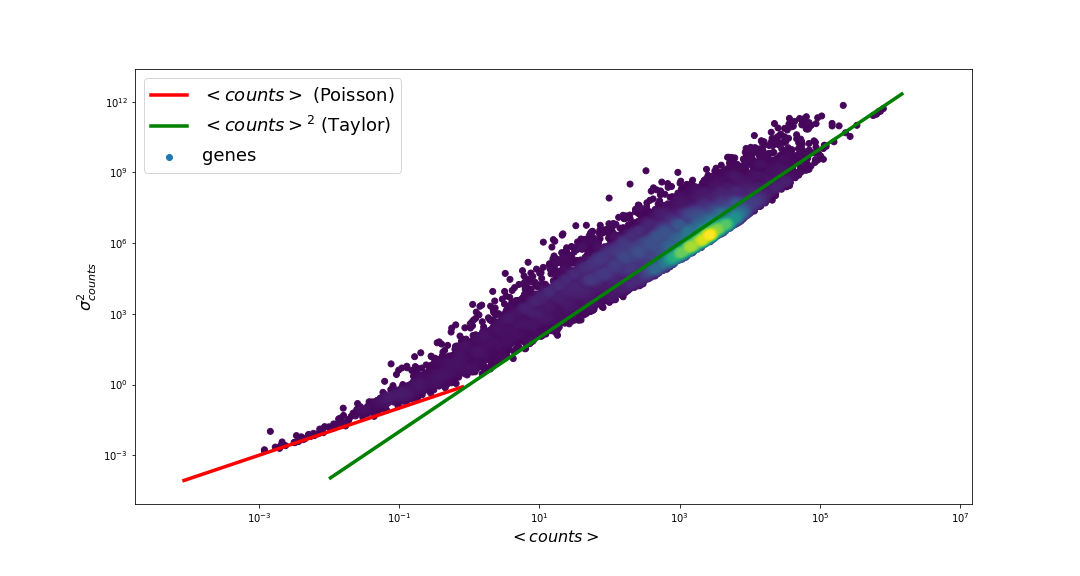
\includegraphics[width=0.9\linewidth]{pictures/scalelaws/gtex/varmean_loglog_density.png}
    \caption{Variance versus occurrence}
    \label{fig:scalelaws/gtex/varmean_loglog_density}
\end{figure}

\begin{figure}[htb!]
    \centering
    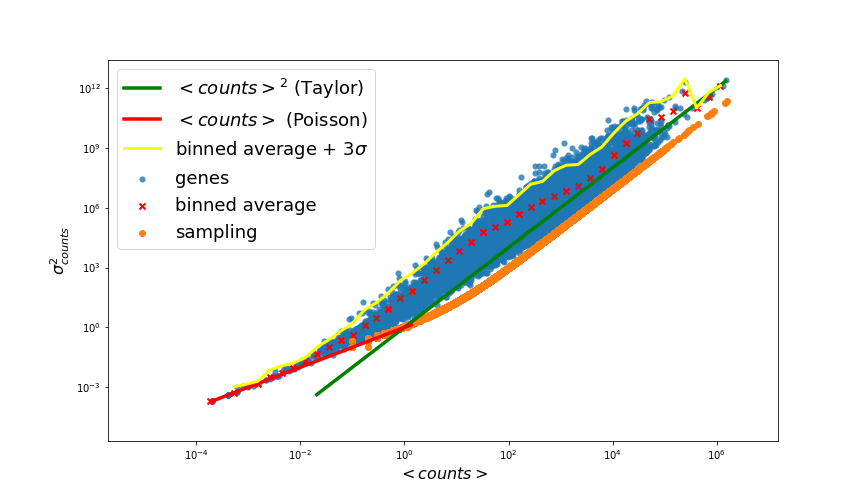
\includegraphics[width=0.9\linewidth]{pictures/scalelaws/gtex/varmean_3sigma.png}
    \caption{Caption}
    \label{fig:scalelaws/gtex/varmean_3sigma}
\end{figure}

\begin{figure}[htb!]
    \centering
    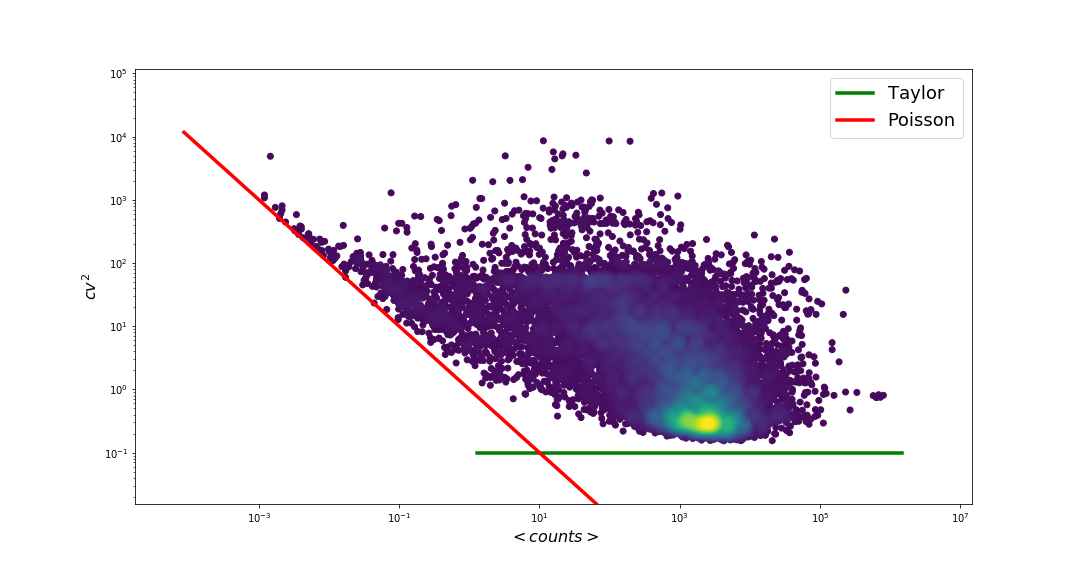
\includegraphics[width=0.9\linewidth]{pictures/scalelaws/gtex/cvmean_loglog_density.png}
    \caption{Variance versus occurrence}
    \label{fig:scalelaws/gtex/cvmean_loglog}
\end{figure}

\begin{figure}[htb!]
    \centering
    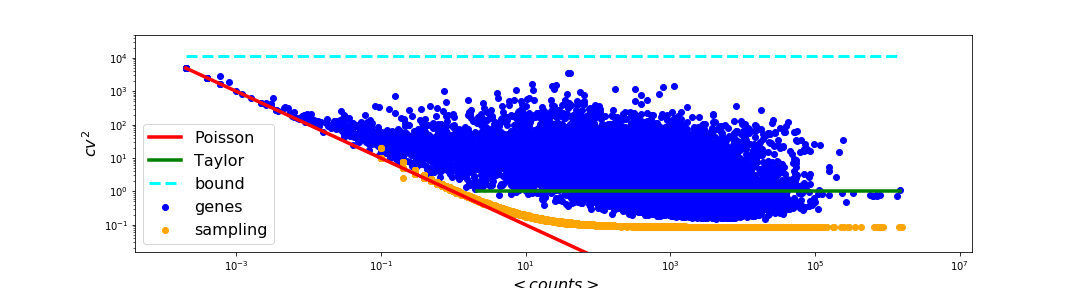
\includegraphics[width=0.9\linewidth]{pictures/scalelaws/gtex/cvmean_loglog_sampling.png}
    \caption{Caption}
    \label{fig:scalelaws/gtex/cvmean_loglog_sampling}
\end{figure}

%%Poisson

%%gamma


\paragraph{$<FPKM>$ versus occurrence}
One can be interested in finding genes that are expressed often, and what is the 
average expression of them.
To manage this it is plotted the average expression $<FPKM>$ versus the number 
of samples in which that gene is expressed that is, considering the thresholds~\ref{sec:threshold}, 
$\Sigma_j\theta (FPKM_{ij}-0,1)\theta (10^5-FPKM_{ij})$

\subsection{Tissue differentiation}
Per gene type scaling

%%GSEA cita

%%gene type distribution


